\documentclass[9pt,twocolumn,twoside]{../../styles/osajnl}
\usepackage{fancyvrb}
\journal{i524} 

\title{Real-time Analysis and Visualization of Twitter data}

\author[1,*]{Sowmya Ravi}
\author[2]{Sriram Sitharaman}
\author[3]{Shahidhya Ramachandran}

\affil[1]{School of Informatics and Computing, Bloomington, IN 47408, U.S.A.}
\affil[2]{School of Informatics and Computing, Bloomington, IN 47408, U.S.A.}
\affil[3]{School of Informatics and Computing, Bloomington, IN 47408, U.S.A.}

\affil[*]{Corresponding authors: sowravi@iu.edu, srirsith@iu.edu, shahrama@iu.edu}

\dates{project-001, \today}

\ociscodes{Real-time streaming, data visualization, Twitter, Natural Language Processing}

% replace this with your url in github/gitlab
\doi{\url{https://github.com/cloudmesh/sp17-i524/tree/master/project/S17-IR-P001/report/report.pdf}}

\begin{abstract}
A real-time system has been developed which extracts live data from twitter, processes the data, calculates a sentiment score based on ensemble of Naive Bayes and Textblob and finally visualizes the sentiment across time and geographical locations. The system has been deployed in chameleon and jetstream cloud platforms. Live data from twitter is injected into the system using tweepy package in Python. Naive Bayes classifier was built in a two-node Apache Spark cluster by training on 3.5 Million tweets. An ensemble of the Naive Bayes classifier and the built-in classifier of Textblob module (Python) were used to determine the sentiment score. The results of the Natural Language processing algorithms were visualized in batches using d3.js and Highcharts.
\end{abstract}

\setboolean{displaycopyright}{true}

\begin{document}

\flushbottom % Makes all text pages the same height

\maketitle % Print the title and abstract box

\tableofcontents % Print the contents section
\maketitle

\section{Introduction}
\begin{figure*}[htbp]
\centering
\fbox{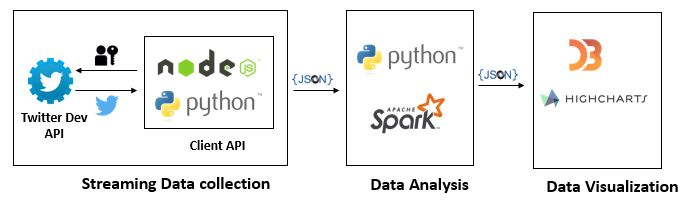
\includegraphics[width=\linewidth, height = 2 in]{images/sysarch}}
\caption{System Architecture}
\label{fig:sysarch}
\end{figure*}
In 1969, Drs. Jerry Boucher and Charles E. Osgood, psychologists at the University of Illinois, proposed the 'Pollyanna Hypothesis' which asserts that "there is a universal human tendency to use evaluatively positive words more frequently and diversely than evaluatively negative words in communicating" \cite{BOUCHER19691}. Such theories were hard to validate due to the absence of significant data and the lack of generality. With Social media turning into the primary platform where people express on a day-to-day basis these claims can be analysed by sampling a portion of the data and applying Natural Language Processing algorithms to determine positivity/negativity of this data. The first step in this process involves extraction of data from Social media using the corresponding APIs. Once the data has been extracted, it is cleaned and restructured to make it suitable for analysis. The results of the Analysis are then visualized in a dashboard to better understand the outcomes.\\
Microblogging website like Twitter is used for analysing behaviour of people because it has emerged to be one of the predominant platforms where people express their opinions about current issues, complain about products, discuss details of on-going events etc. Twitter data also aids in understanding behavioral patterns across diverse demographics - location, gender etc. Twitter generates nearly 200,000 tweets in less than a minute \cite{www-twitstat}. This large sample of data can then be used to test the hypothesis. Big data technologies prove to be particularly useful in storing, processing and analysing such large data sets. It also makes it possible to setup real-time systems that can output results with a latency of very few seconds. \\
he data for the system was extracted from Twitter using it's API through Python. This data is processed and manipulated in Python and PySpark which is finally visualized using D3.js and Highcharts. The remainder of the paper is organised as the System Architecture, Work flow, Deployment, Benchmarking and Conclusion. \section{System Architecture}
The streaming pipeline for analysing the data consists of different components to aid in different stages of the analysis. The architecture of these components have been elaborated in this section. The system architecture is shown in the Figure \ref{fig:sysarch}.
\subsection{Python}
Python was primarily used for tweet extraction, pre-processing and analysis. Various packages were used to aid in the process. 'Tweepy' package\cite{www-tweepy} was used for extracting tweets directly from Twitter API. The user has to create an application by logging into the tweepy portal and using the unique access tokens and cosumer keys he/she can access the data from Twitter. OAuthHandler module assists in accessing the data securely. StreamListener module is used to directly extract the tweets from Twitter. 'JSON' library \cite{www-json} was used to handle the JSON data output from tweepy and to provide as input to highcharts and D3.js. 'Pandas' \\cite{www-pandas}, which is Python's data analysis library was used for manipulating the data while pre-processing. 'Numpy' \cite{www-numpy} package was used for data handling. 'zipcode' \cite{www-zipcode} package was used to extract geographical data for visualizing on maps. 'NLTK' \cite{www-nltk} package was used for building classification model through 'Textblob' module \cite{www-textblob}. 'wordcloud' \cite{www-wordcloud} and 'matplotlib' \cite{www-matplotlib} were useful in creating wordclouds of the positive and negative tweets.   
\subsection{Apache Spark}
Spark provides a distributed cluster computing framework for processing large amounts of data. The architecture of spark is shown in Figure ~\ref{fig:spark_arch}
The  Spark system encompasses a Master/ Driver and Workers. The Master contains the Spark context which serves as the execution environment for Spark. Each worker node contains one or more executors which run processes. The driver manages all the workers via an external processes like YARN or Mesos \cite{www-apache_spark}. 
Spark supports multiple languages which include Scala, Java, Python and R. In addition to the spark core framework , it has an Application Programming Interface for Streaming (Spark Streaming), SQL(Spark SQL), Machine Learning(Spark MLLib) and graph computation (Spark GraphX). \\
\begin{figure}[htbp]
\centering
\fbox{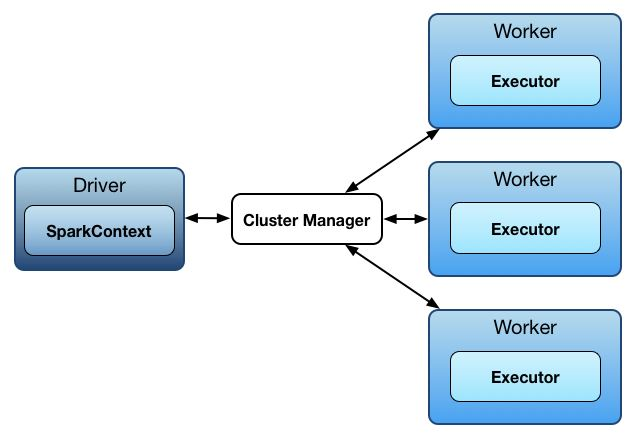
\includegraphics[width=\linewidth]{images/spark_arc}}
\caption{Architecture of Apache spark}
\label{fig:spark_arch}
\end{figure}
Spark is built on Hadoop and it uses the Hadoop Distributed File System(HDFS) for Data Storage. It can also access diverse data sources including Cassandra, HBase, and S3. Spark stores the data in the form of Resilient Distributed Data(RDD). RDD is the basic data storage unit in spark. They are read-only, logically partitioned collection of records and they are stored in a fault-tolerant manner.  Each partition in an RDD may be stored and computed at a different node. RDDs are created in two ways: one is by paralleling an existing collection and the second is by referencing an existing data set\cite{www-RDD}.\\
The spark can be operated in either Standalone mode or in cluster mode. While operating in cluster mode, spark makes use of YARN framework for resource management and distributed computing. The YARN is responsible for allocating tasks, delivering data to the worker nodes and collecting the results of the process. 
\subsection{Node.js}
Node.js is an open source, asynchronous, Javascript run-time environment which enables JavaScript to be used for server side scripting \cite{www-nodejs}. It has an event driven architecture that focuses primarily on throughput and scalability of web applications. It works based on callbacks rather than threading to signal completion of tasks. Though it does not support threading it allows ,multi-core  usage through child processes. The cluster modules aids in balancing load across the cores. Node.js combine JavaScript with Unix network programming in order to provide concurrency without compromising on performance of the server side program. It is comparable to systems like Ruby's Event Machine or Python's Twisted. In Node.js there is no mechanism to explicitly call the event loop start. The event loop is entered after the input script is executed and exited when there are no more callbacks. It is commonly used for running server side web applications to produce dynamic web page content before the page is sent to the user's web browser.
\subsection{D3.js}
D3.js is a JavaScript library for manipulating website elements based on user data. D3 uses using HTML, SVG, and CSS for rendering the web page \cite{www-d3-web}. It combines powerful visualization components thereby providing a data-driven approach to web-page DOM (Document Objects Model) manipulation. D3.js offers flexibility by exposing the full capabilities of web standards such as HTML, SVG, and CSS. With minimal overhead, D3 is extremely fast, supporting large data-sets and dynamic behaviors for interaction and animation. It works by selecting elements of a HTML webpage and adding an svg element on top of it. The SVG element can vary through a series of objects like a rectangle, circle, text etc. Each of these objects has their own attributes defining their shape, label, position etc. in the web page. These shapes can also be styled by using a style class in a CSS file. Hence, D3.js in a nutshell accesses HTML, CSS and SVG components of a web page which makes rendering visualization of data in an efficient, simple and fast manner.
\subsection{Highcharts}
Highcharts is an online Data Visualization product created by the Highsoft team based out of Norway \cite{www-highwiki}. It is a charting library written entirely in JavaScript. It allows creation of interactive visualizations that can be hosted on web pages or web applications. The data to be visualized is input as JSON file. as input data Highcharts currently supports line, spline, area, area-spline, column, bar, pie, scatter, angular gauges, area-range, area-spline-range, column-range, bubble, box plot, error bars, funnel, waterfall and polar chart types  \cite{www-Highcharts}.
\section{Work flow}

\subsection{Cloudmesh Client}
Cloudmesh is a cloud management client that provides seamless integration to multiple clouds from command line. Some of the features of cloudmesh include heterogenous cloud integration, deployment of hadoop cluster with add-ons such as spark and pig \cite{www-cm-git}. It also enables automated builds 

\subsection{Ansible}
Ansible is a powerful IT automation engine that helps in the deployment of of applications. It doesn't use any customized security infrastructure that and it is very easy to deploy. The YAML, a simple language, is used to write ansible scripts. The main component of the ansible is a playbook which is YAML file that contains all the processes and applications that have to be deploys in the remote system \cite{www-ansible}. \\
Ansible pushes small chunks of code called modules that are executed on the nodes. These modules are executed over ssh by default and removed once they are completed. Also, these modules can reside anywhere and d not require the use of database systems , servers or daemons \cite{www-ansible}.\\
Ansible supports the use of ssh keys as well as passwords. However, ssh keys are relatively simple to use. Another noteworthy feature of ansible is that root logins are not required and later one can sudo to any user. The Ansible authorized key module is an efficient way to control other hosts. Additional options such as kerberos or identity management systems are also available for use \cite{www-ansible}. \\
The Playbook is the heart of an ansible work flow. The playbook enable the user to control the infrastructure details of the project such as the number of machines to be considered for the task and the processes to be deployed in each of those machines \cite{www-ansible}. A basic ansible playbook is shown in Figure \ref{fig:playbook} 
\begin{figure}[htbp]
\centering
\fbox{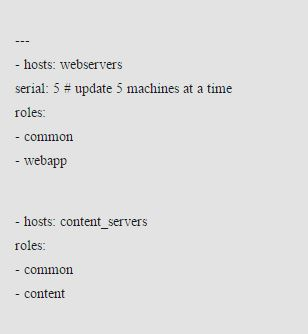
\includegraphics[width=\linewidth, height = 2.5 in]{images/playbook}}
\caption{Structure of an Ansible Playbook \cite{www-ansible}}
\label{fig:playbook}
\end{figure}
The list of hosts is usually provided in a file and each group of hosts is usually given a name that is later reference in the playbook. While running an ansible playbook, the inventory/host file is also passed in the command. Logging into machines do not require an SSL signing in. A sample ansible inventory is shown in Figure \ref{fig:inventory}. 
\begin{figure}[htbp]
\centering
\fbox{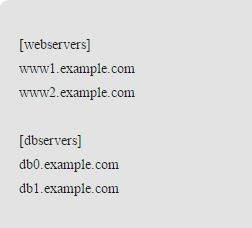
\includegraphics[width=\linewidth, height = 2 in]{images/inventory}}
\caption{Structure of an Ansible Inventory \cite{www-ansible}}
\label{fig:inventory}
\end{figure}
\subsection{Tweet Extraction}
Python is used as the platform for collecting real-time data from Twitter. Using the 'tweepy' package, a tweet extracting module was built which authenticates the collection of data from Twitter's API. This is done by using the 'Consumer key' and an 'Access token' generated by Twitter's developer API. This Consumer key and access token are unique to the application created by the user. Of the total number of tweets authored in Twitter at a given time, only 1\% -2\% of the tweets can be extracted. Of these tweets that were extracted, only 1\% -2\% of the tweets are geo-tagged. While extracting the tweets, filter was applied on Language to extract only those that were authored in 'English' language. Tweets were collected at the rate of generation as a JSON object in Python. the data was not stored in a RDBMS/ NoSQL database since data files in the Gigabytes range slowed down the system when implemented in Chameleon cloud platform. Instead, batch processing technique was used, where the tweets were extracted and processed in batches. The results of analysis of this batch of tweets were then visualized. The results of each of the subsequent batches were aggregated with the previous batch in Python. The visualizations were also subsequently updated. 
\subsection{Tweet Pre-Processing}
Since the extracted tweets were in JSON format, they had to be pre-processed in order to be used for analysing and calculating sentiment scores. The various steps in pre-processing have been elaborated in this section. 
\subsubsection{Parsing}
The data had to be parsed to get convert the data in JSON format to a pandas data frame with columns populated with : textual content, location, country code, country name, state code, time of generation etc. The missing values were replaced with 'NA's. 
\subsubsection{Tokenization}
A custom tokenizer was built that does not separate the hashtags $\#$ from the word. Similarly, $@$ and the textual part of the mentions were retained as a single entity. Other special cases included retaining all the characters in emoticons together as a token, extracting URLs together etc. After testing the performance of the tokenizer manually, the datasets were given as input to the tokenizer. Files with a single token on each line and an empty line following each tweet were created.
\subsubsection{Word Vector Creation}
For each of the tweets, word vector files were created which includes the tokens from the tweets as individual features and values were given based on their presence in each tweet. The value for that respective column was set to be 1 if the word/token was present in the tweet and 0 otherwise.
\subsubsection{Feature Engineering }
Two lexicons were provided: Arguing Lexicon and MPQA subjectivity lexicon. Features were created from each of these lexicons for the train and test data-set of each target. 

\begin{itemize}
\item{\textbf{Arguing Lexicon:}
Arguing lexicon \cite{somasundaran2007detecting} is a hand built lexicon built by Somasundaran, et al., contains 17 “.tff” files describing patterns that represent arguing. Each file contains patterns that are specific to one type of argument. For instance, “authority.tff” contains patterns that might occur in the text that involves a person or an entity exhibiting authority in some manner. There are certain areas in the pattern files that contain words that start with “@”. The corresponding definition for these words were given in 5 macro files. Modals, Spoken, Wordclasses, pronoun and intensifiers are included in the 5 macro files. For example, in “emphasis.tff” there is a pattern “(@GONNA)”, the value of which is present in the “modals.tff” macro file. 
\begin{center}
"@GONNA": ["am going to"," are going to"," is going to"," am gonna"," are gonna"," is gonna"]
\end{center}
Here, “@GONNA” was replaced by the corresponding list of values shown above. It can be any one the listed values. \\
All the 17 files were read in python as a list of patterns. Macro files were used to replace the macros present in these 17 files wherever necessary. Regex package in python was used to read and compile each pattern in each of the 17 files as regular expressions. 17 new features were created and 0/1 values were assigned if a text contains at least one regular expression from the list for each lexicon file. The created feature would have the value 1 if any one of the regular expression has a match with the input tweet, otherwise 0. This process was repeated for all the targets’ train and test data-sets.}

\item{\textbf{MPQA subjectivity lexicon} was also used in the process of creating new features. This lexicon contains a clue file which was developed by Riloff and Wiebe, 2003 as a part of their work in subjectivity expressions \cite{riloff2003learning}. The clues in the file were provided in the following format:
\begin{center}
type=strongsubj len=1 word1=abuse pos1=verb stemmed1=y priorpolarity=negative
\end{center}
A clue that is subjective in most context is considered strongly subjective (strongsubj), and those that may only have certain subjective usages are considered weakly subjective (weaksubj). “Word1” denotes the token or stem of the clue, whereas “pos1” denotes the part-of-speech of the corresponding word. Apart from subjectivity, the polarity of the word whether its positive, negative, neutral or both is given by “priorpolarity”.}
\end{itemize}
\subsection{Classification Model}
\subsubsection{NLTK - Textblob}
Textblob is a python wrapper(for python 2 and python 3) class of the NLTK package. It provides various modules for utilizing the functions of NLTK. Hence, the usage requires NLTK and all NLTK corpora to be installed initially. The sentiment analyser tool in textblob gives the polarity when a sentence is given as input. It can recognize several different languages. 
\subsubsection{PySpark with NLTK}
Spark framework comes with a powerful Machine Learning API called MLLib. The MLLib contains predefined functions for popular machine Learning Algorithms. The NaiveBayes classifier was used along with the python's NLTK toolkit to get the sentiments associated with each tweet. The resulting model was stored in a the local file system.  Each subsection describes the functions and modules used to build the Naive Bayes Classifier.\\
The output of tweet extraction is read by the Spark Context using a JSON reader. The data is then pre-processed and cleaned by removing the stopwords from the tweets. The tweets then  tokenized using the NLTK tokenizer. The tokenized tweets are used to create feature vector with  features using the hashing trick. Hashing maps the data of an arbitrary size to a fixed size which is 50000 in this case. A Labelled Point vector which is a type of RDD with the label and feature vector as a key value pair. The Labelled Point vectors are useful in training supervised algorithms in MLLib. Sixty percent of the Labelled point data was used for training the Naive Bayes Classifier. The model obtained as a result of training is stored in the local file system. The model is tested on the remaining data. The predictions along with the correct labels are also stored locally in file. To process and manipulate the data the classic Hadoop functions such as Map, FlatMap and Filter were used. The functions are described in the upcoming sections.
\begin{itemize}
    \item \textbf{Map}: Map applies a function to all the elements of a RDD. This is achieved in PySpark by using Lambda functions. 
    \item \textbf{FlatMap}: Flat Map is similar in function to map however  , it transforms an RDD to a collection and then back t an RDD. The results in a flattened output. The input and output RDDs can be of different sizes. 
    \item \textbf{Filter} The filter applies a condition to every row of an RDD and retains rows that satisfies that condition.
\end{itemize}
\begin{figure}[htbp]
    \centering
    \fbox{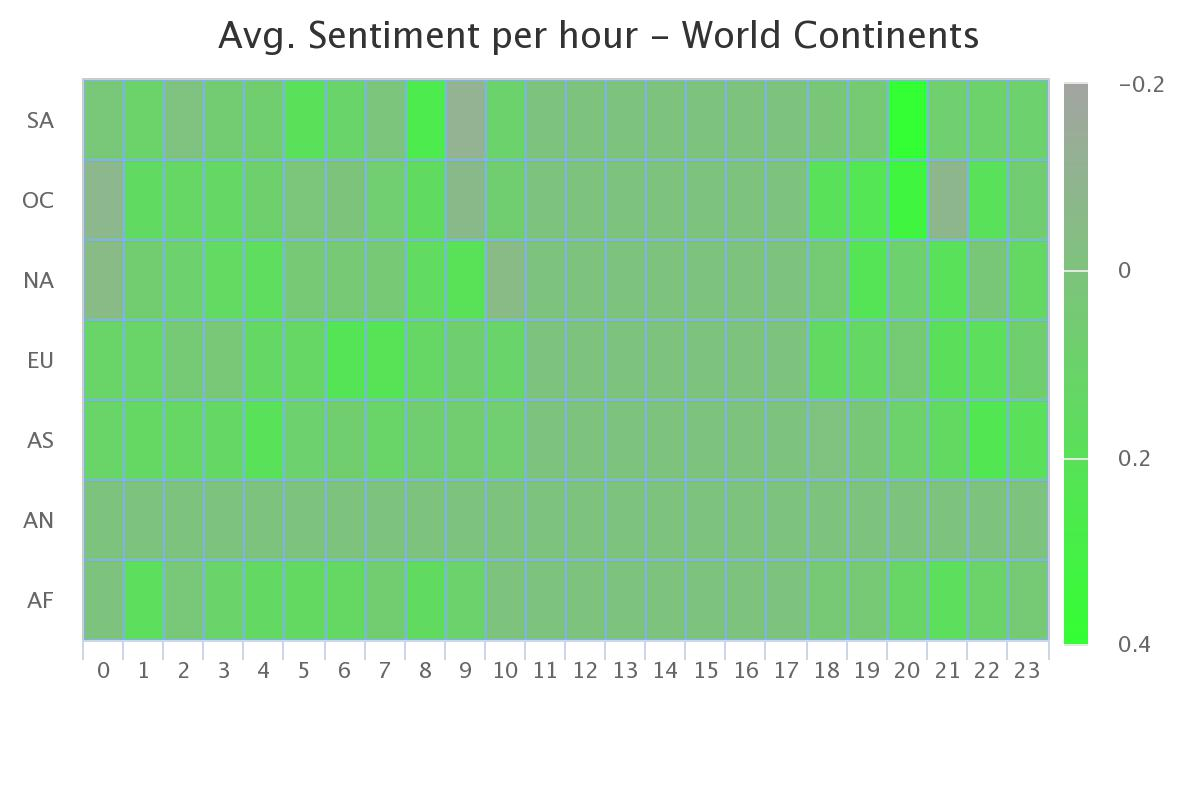
\includegraphics[width=\linewidth, height = 2.5 in]{images/senticont}}
    \caption{Tweets Count - Time}
    \label{fig:tweetsenti}
    \end{figure}
\subsection{Data Visualization}
Data Visualization is an integral part of the sentiment analysis of Twitter data. Visualization tools such as D3.js and Highcharts \cite{www-Highcharts} have been used to visualize the data.Visualizations created using Highcharts are updated as batches of tweets are extracted and processed in real-time. These charts change dynamically as each batch of tweet data gets processed over time. Visualization created using D3.js is directly connected to the Twitter API and thus it gets updated without any latency. A series of visualizations have been created in D3.js and Highcharts to analyze the data and project results of NLP analysis onto geographical and temporal spaces. The section below elaborates on the visualizations implemented.
    \begin{figure}[htbp]
    \centering
    \fbox{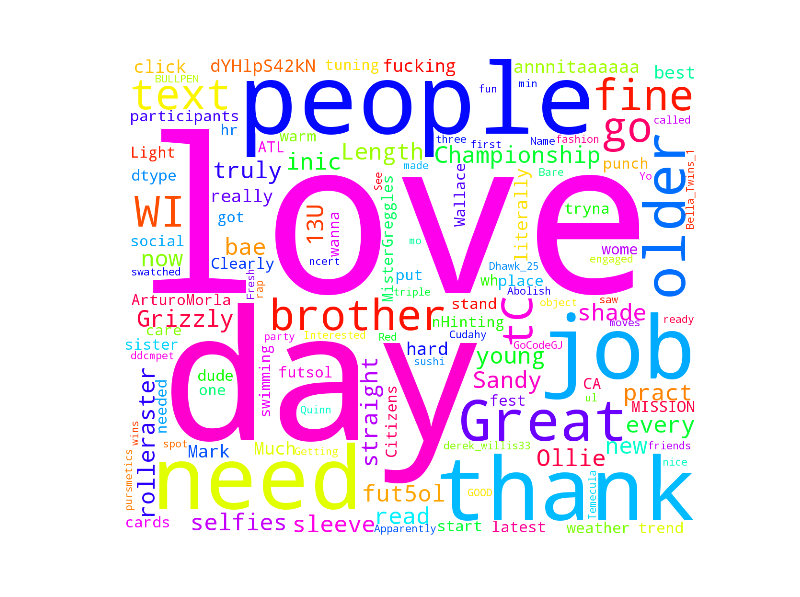
\includegraphics[width=\linewidth, height = 2.5     in]{images/postive}}
    \caption{Word Cloud for Positive tweets}
    \label{fig:poswordcloud}
    \end{figure}
\subsubsection{Temporal Analysis}
To analyze the data with respect to time, the tweets were aggregated with respect to the time stamp. The tweets generated all over the world were collected by filtering on 'English' language. The number of tweets generated from each country was plotted along the time axis to identify the period of time during the day when people tweeted the most. A matrix was created to understand the average positivity/ negativity/ neutrality of people around the world during different times of the day. 
\begin{itemize}
    \item \textbf{Count of Tweets generated vs Time:}\\
    \begin{figure*}[htbp]
    \centering
    \fbox{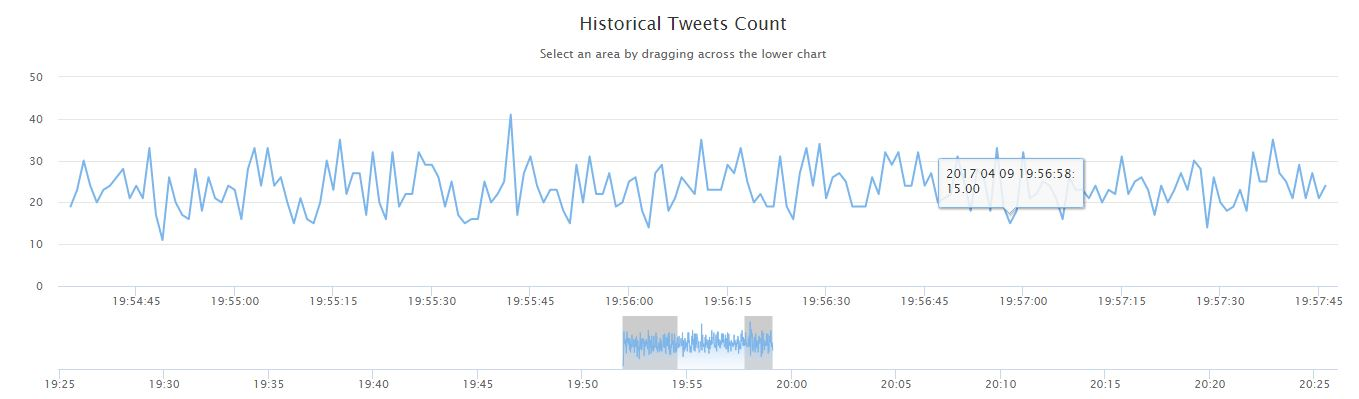
\includegraphics[width=\linewidth, height = 2.5 in]{images/timechart}}
    \caption{Tweets Count - Time}
    \label{fig:tweetcnt}
    \end{figure*}
    The plot of the number of tweets generated in a given period of time is shown in figure \ref{fig:tweetcnt}. Line chart has been used because it clearly depicts the trend in number of tweets in a given second. The time (in UTC) is plotted along the horizontal axis and the number of tweets is plotted along the vertical axis. In the figure \ref{fig:tweetcnt}, the number of tweets have been plotted for the time period $19:54:30$ to $19:58:00$ on April 09, 2017. It is possible to select the time range for which we want to see the trend in more detail by clicking and dragging the mouse in the horizontal axis \cite{www-HCMasterdetail}. The tool-tip gives information about the exact time-stamp and the corresponding number of tweets generated at that time. The plot can be used to observe the peaks in activity in Twitter over a period of time. 
    \item \textbf{Average Sentiment across Continents vs Time:}\\
    The chart giving the sentiment score as a function of continent and time is shown in the figure \ref{fig:tweetsenti}. Each block in this matrix gives the average sentiment in a particular continent at a particular time \cite{www-contisenti}. The continents are given along the horizontal axis and the time periods are mentioned along the vertical axis. The tool-tip gives information about the time-period and the average sentiment score corresponding to each Continent. Since tweets are generated from as many as 180 countries, the analysis has been aggregated at the Continent level in order to obtain an overall picture. This chart depends on the sample of data chosen for plotting and hence it becomes essential to choose a stratified sample that is representative of the actual population. This can be ensured by choosing a significant number of tweets from each of the continents for the analysis. From the plot, it is seen that most tweets are generated during 7:00 AM to 9:00 AM and 19:0o Pm to 22:00 PM periods of time. Also, American continents are more active on Twitter as compared to the Asian and African continents. 
\end{itemize}
\subsubsection{N-grams Analysis}
In a Natural Language Processing model, n-grams form important features in identifying the sentiment of a  given text. N-grams can be word unigrams, bigrams, trigrams or they can also be character unigrams, bigrams, trigrams. Since the scale of Twitter data is very large word n-grams have been used for the sentiment analysis. As part of the n-gram analysis, Co-occurrence of word pairs in tweets and the most commonly occurring word unigrams in positive and negative tweets have been visualized. 
    \begin{figure}[htbp]
    \centering
    \fbox{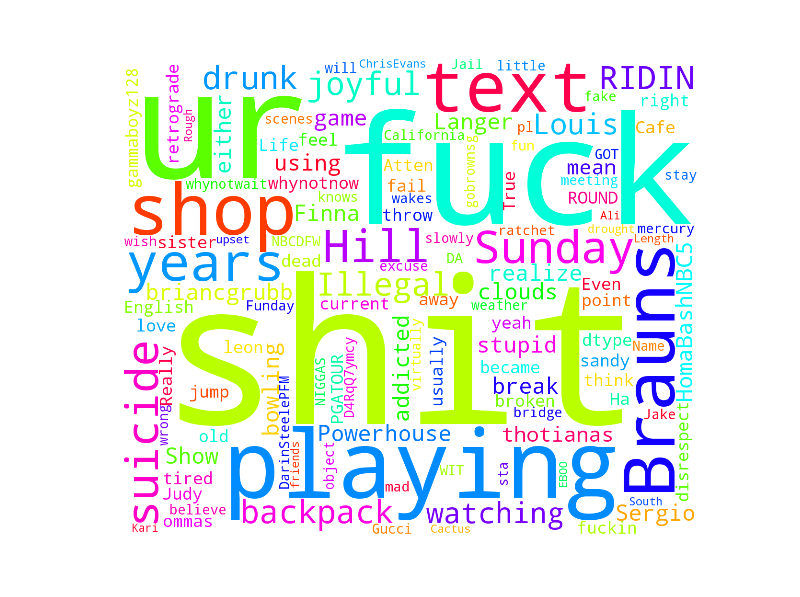
\includegraphics[width=\linewidth, height = 2.5     in]{images/negative}}
    \caption{Word Cloud for Negative tweets}
    \label{fig:negwordcloud}
    \end{figure}
\begin{itemize}
    \item \textbf{Word Co-occurrence Matrix:}\\
    \begin{figure*}[hbt]
    \centering
    \fbox{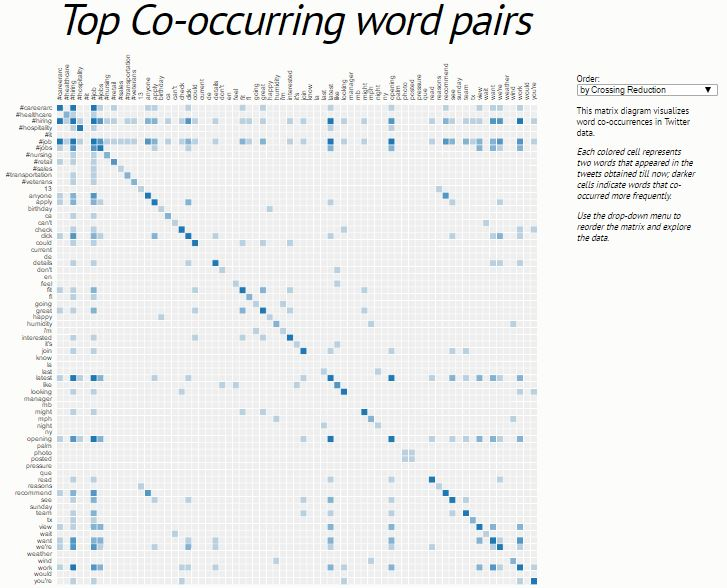
\includegraphics[width=\linewidth, height = 4     in]{images/cooccur}}
    \caption{}
    \label{fig:wordcooccur}
    \end{figure*}
    In Natural Language Processing, bigram combinations are used as features while developing a Sentiment Analysis model. This chart gives the co-occurrence patterns for the top 200 commonly occurring word pairs. All possible combinations of pairs of words belonging to a tweet were considered. Based on the number of times these word pairs had occurred in the tweets collected, the top 200 most commonly occurring pairs were determined. The probability co-occurrence of these word pairs were then projected onto a matrix \cite{www-cooccur} as shown in the Figure \ref{fig:wordcooccur}. This is an interactive plot where the order in which the words are displayed can be altered based on the Name, Frequency of occurrence, cluster, spectral \cite{www-reorder} etc. The probability of co-occurrence has been differentiated by varying the intensity of blue used in the pixel corresponding to the pair of words. The darker the shade of blue greater is the probability of the two words occurring together in a given tweet. From the plot, it can be seen that the words like 'job', 'hiring', 'careerarc', 'work' etc. have high probability of co-occurring with each other. 
    \item \textbf{Word Cloud:}
    Separate word clouds were created for tweets tagged as having a positive sentiment and those tagged as having a negative sentiment. Based on the NLP model built, a certain sentiment score was calculated for each tweet based on the n-gram features. This sentiment score value ranges from -1 to +1. Positive score indicates positivity of the tweet and negative score indicates negativity of the tweet. A score of '0' was considered as a neutral tweet. The tweets with negative and positive scores were aggregated separately and the word unigrams were plotted in a word cloud. The word cloud displays a collection of words occurring in the data \cite{www-wordcloud}. The size of the word is directly proportional to the frequency of its occurrence in the data. From the positive wordcloud shown in Figure \ref{fig:poswordcloud}, it can be seen that words like 'love', 'thanks', 'fine' etc. have been frequently used. The negative wordcloud shown in Figure \ref{fig:negwordcloud} clearly projects abusive words commonly used in tweets which in most cases are indicative of the sentiment.     
\end{itemize}
\subsubsection{Analysis for US-States}
US is one of the major locations from where a significant number of tweets are generated. In the data that was collected from Twitter for the purpose of analysing sentiment, it was observed that majority of the tweets were from USA. Thus, Visualizations were created for analysing the amount of tweets generated and the average sentiment conveyed by these tweets across the states of the USA. Highmaps \cite{www-highmaps} were used for visualizing this data, where the values were projected onto the geographical map of US based on the latitude and longitude information. Heat maps have been used to represent this data, where the intensity of color is used to differentiate the value across multiple regions. \begin{itemize}
    \item \textbf{Number of tweets in US States:}\\
    From the Figure \ref{fig:ustweet}, one can see the number of tweets generated across the different states in the US. For the geo-tagged tweets available in the data, the country of tweet generation was extracted. Those tweets with Country code as 'US' were filtered and the state code was extracted for these tweets. The state code was then used to map the latitude-longitude information for each of the states. The number of tweets generated was aggregated at the State level. This was then used as JSON input to generate the graph in Highmaps \cite{www-uscount}. The color scale shown at the bottom of the graph gives the intensity of Blue used for different frequency ranges. The number of tweets generated from each state has been projected on to the corresponding geographical location. This has been developed as an interactive graph, where particular regions can be zoomed to get a clearer view of the distribution. From the graph we can see that there is more activity along the coastal regions of the US as compared to Northern states of America. it can be seen that most tweets are generated from California on the West coast and majority of tweets are generated from the East coast of USA.  
    \begin{figure}[htbp]
    \centering
    \fbox{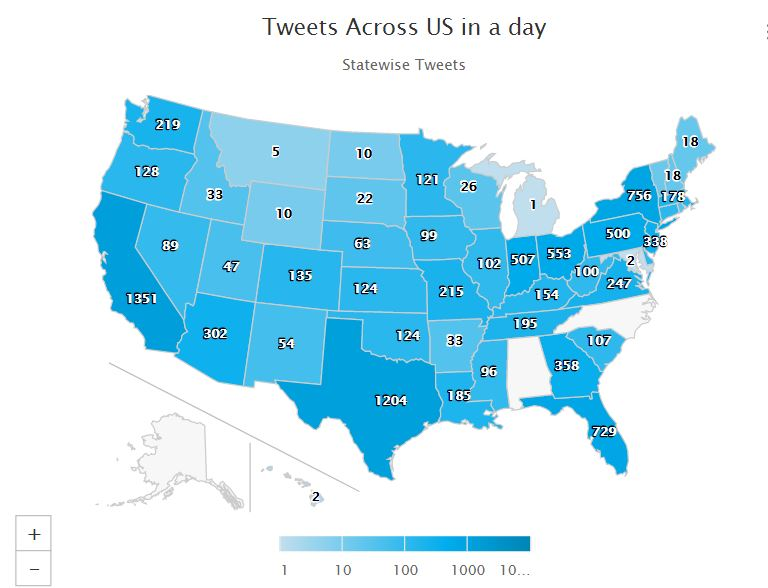
\includegraphics[width=\linewidth, height = 2.5     in]{images/us_tweet}}
    \caption{Number of tweets in US States}
    \label{fig:ustweet}
    \end{figure}    
    \item \textbf{Average Sentiment across US States:}\\
    The average sentiment across the various states of US was visualized as shown in the Figure \ref{fig:ussenti}. Data was extracted using a procedure similar to that explained in Section 4.3.1. The average sentiment score was calculated by taking average of the sentiment scores of all the tweets from a given state. This graph was also developed as an interactive graph, where one can zoom into regions of interest for better understanding. The color corresponding to each class (Positive/Negative/Neutral) is shown at the bottom of the plot. In addition to creating a heat map for understanding the majority sentiment, pie charts were imposed onto the states to provide the percentage distribution of negative, positive and neutral tweets \cite{www-ussenti}. The heat map assigns the color of majority class to the state. In this way, the majority region of the pie chart will be indistinguishable from the background and one can see the distribution of other two classes in the same state. From the graph , it can be  seen that majority of the states have neutral sentiment. The pie charts show that, though most states have a neutral sentiment, some states are less negative than the others.
    \begin{figure}[htbp]
    \centering
    \fbox{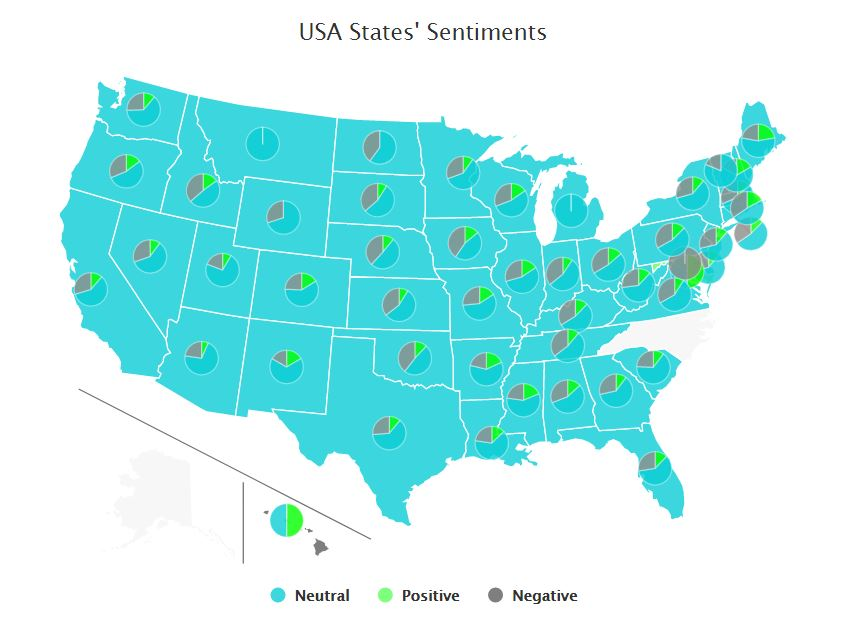
\includegraphics[width=\linewidth, height = 2.5 in]{images/us_senti}}
    \caption{Average Sentiment across US States}
    \label{fig:ussenti}
    \end{figure}    
\end{itemize}  
\subsubsection{Analysis for World Countries}
All tweets with geo-location information were analysed to understand the amount of tweets generated and their average sentiment with respect to countries. These values were then projected onto the world-map to identify regions of high activity and regions of positive, negative or neutral sentiment. The first graph displays real-time generation of tweets by highlighting the country from where it is generated. The latter is a heat map displaying the average sentiment across world countries in the map.
\begin{itemize}
    \item \textbf{Number of tweets in World Countries:}\\
    \begin{figure}[htbp]
    \centering
    \fbox{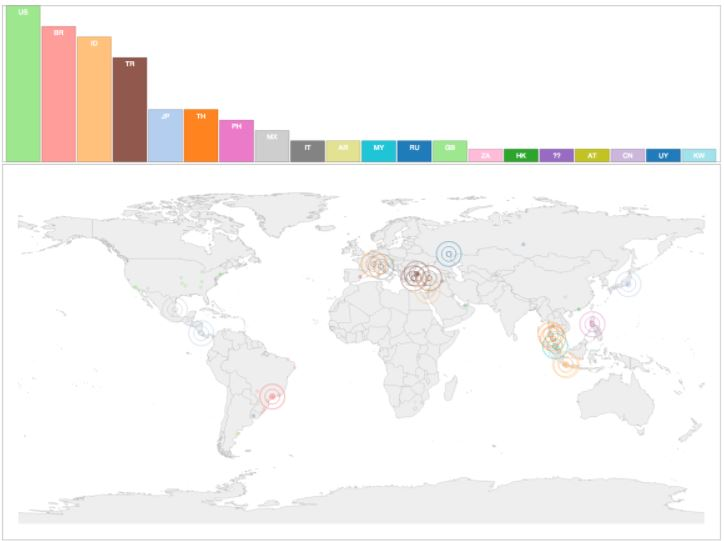
\includegraphics[width=\linewidth, height = 2.5     in]{images/realtime}}
    \caption{Number of tweets in World Countries}
    \label{fig:worldno}
    \end{figure}
    Figure \ref{fig:worldno} shows the number of tweets generated in each country. This visualization was developed as a combination of bar chart and the geographical map. It was created using D3.js by obtaining the JSON data from node.js \cite{www-d3}. The visualization directly connects with the Twitter API in real-time with a delay of 2-3 seconds. Each geocoded tweet is visualized as a point of longitude and latitude on the map. When a tweet is generated, it is indicated by animated concentric circles around that point. After the animation ends it is marked by a dot with color corresponding to the color of the country in the bar chart. In parallel, a counter tracking number of tweets generated from the corresponding region is incremented and plotted on the bar chart. Only top 20 countries in terms of tweet generation are visualized in the bar chart. The country code is specified at the top of the corresponding bar. From the plot, it can be seen that maximum number of tweets are generated from US, which is in line with what was observed in the data collected.
\end{itemize}
\section{Deployment}
\subsection{Hadoop and Spark}
Cloudmesh was used to deploy Hadoop and spark in the Virtual machines. A cluster with three nodes were created. One of the machines served as the master while the other two machines were the worker nodes. Two playbooks were created: the first playbook was used to install cloudmesh client and the second playbook was used to deploy a hadoop cluster with spark as an add-on. An overview of the tasks performed by the ansible playbook  that deployed a hadoop cluster with spark in 3 virtual mahines is detailed below.
\begin{enumerate}
    \item Virtualenv and Virtualenv wrapper were installed
    \item the python dependencies for cloudmesh were installed.
    \item Dependencies for cloudmesh client were installed
    \item Install cloudmesh client in the local system
    \item Generate ssh key if it doesn't exits
    \item A default cloud was selected
    \item The ssh key was added to cloudmesh
    \item The security group was uploaded into cloudmesh
    \item A cluster with three nodes was defined 
    \item Hadoop was deployed using spark as an add-on 
    \item The cross ssh connection between the three nodes was verified to enable communication between the nodes.
\end{enumerate}

\subsection{Implementation of Naive Bayes Classifier using spark MLLIb}
The code for the Naive Bayes classifier was uploaded in a common repository in github. An ansible script was written that fetched the code and executed it inside the master node. The model and the classified results were saved inside the master node's Hadoop distributed File system. This file was later pushed to a git repository which further utilized the results to create visualizations using D3.js

\subsection{Analysis of Tweets using Python}
Python was used to extract tweets from the twitter and the following packages of python was used for performing the multiple text analysis mentioned
\begin{enumerate}
    \item Tweepy
\item Pandas
\item TextBlob
\item Numpy
\item Zipcode
\item matplotlib
\item nltk
\end{enumerate}

The version of Python used was 2.7x. \textbf{Ansible-node} role was used to install python and its dependencies, followed by the installation of pip which was used to install the python packages mentioned above.
\subsection{Visualization components}
Two components of visualization was deployed. One using nodejs and d3.js for visualizing the tweets in their geo location in a world map. Another is the set of charts and maps using Highcharts visualizing the results of the analysis performed in the previous step.Later part of the \textbf{Ansible-node} role was used to install nodejs and its dependencies, and start the python http server for viewing the visualizations.  
\begin{table}[htb]
\centering
\caption{Chameleon cloud Specification}
\label{tab-cham}
\begin{tabular}{@{}clll@{}}
\toprule
\textbf{Value}    & \multicolumn{1}{c}{\textbf{Chameleon}} \\ \midrule
\textbf{group}    & default         \\
\textbf{secgroup} & default  \\
\textbf{image}    & Ubuntu-Server-14.04-LTS\\
\textbf{flavor}   & m1.medium    \\ \bottomrule
\end{tabular}
\end{table}
\section{Benchmarking}
Benchmarking was done to evaluate and compare the performance of the system by varying the Cloud environment, cluster set-up, algorithms and data sizes. Benchmarking was also done on system performance in local machines. Local machine used was dual core machine with 8 GB RAM and 64bit OS. The configuration of the machines on which the analyses were run is as given below:
The system was deployed in Chameleon cloud platform. The virtual machines used for the analysis had the following configuration:\\  

\subsection{Naive Bayes vs NLTK-Textblob}
Two different algorithms were used to classify the tweets based on positive, negative or neutral sentiment. Naive Bayes classifier was developed in PySpark and the saved model was used for the classification task. The model was built on annotated training data and tested on data extracted from Twitter. Textblob module of the NLTK package in Python was also used for classifying the tweets. The performance of both the machine learning models were verified on a common validation set. Table \ref{tab-acc} gives the accuracies of the two models on 10,000 tweets extracted from Twitter and annotated manually. Since Textblob had better accuracy than Naive Bayes classifier, all the analyses were done based on the sentiment scores determined using Textblob. 
\begin{table}[htb]
\centering
\caption{Accuracy of ML models}
\label{tab-acc}
\begin{tabular}{@{}cc@{}}
\toprule
\textbf{Model}               & \textbf{Accuracy} \\ \midrule
\textbf{NLTK-Textblob}       & 62.81\%           \\
\textbf{PySpark-Naive Bayes} & 51.36\%           \\ \bottomrule
\end{tabular}
\end{table}
\subsection{Chameleon}
Chameleon cloud was one of the three platforms used for deploying the real-time system. The time taken for installation of dependencies and the time taken for execution of the algorithms were recorded. Textblob tweet analyses was done using Python in a single cloud virtual machine. To run this analyses all package dependencies like Pandas, TextBlob, Numpy, Zipcode, matplotlib, nltk and node.js had to be installed in the cluster. Time taken to determine the sentiment score of tweets using textblob is shown in Figure \ref{fig:tbrun}.\\
\begin{figure}[htbp]
\centering
\fbox{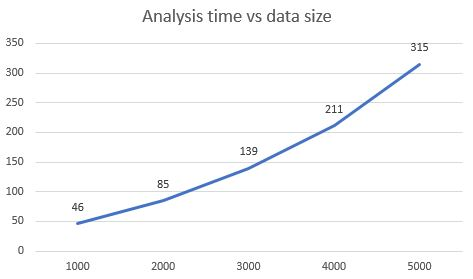
\includegraphics[width=\linewidth, height = 2     in]{images/tbrun}}
\caption{Run time of Textblob}
\label{fig:tbrun}
\end{figure}
The Naive Bayes classifier built in PySpark was implemented in multiple nodes within a cloud Virtual machine. To implement this model, Hadoop, Spark and HDFS had to be installed in each of the nodes in the cluster. As clearly seen from the Table \ref{tab-chamtime} PySpark takes longer time to to get executed as compared to Textblob due to the parallel processing of data. Also, the installation of dependencies take significant amount of time as compared to the system execution. Figures \ref{fig:chamstat1}, \ref{fig:chamstat2} and \ref{fig:chamstat3} give the run time of implementing the classifier in a cluster with 1,2 and 3 worker nodes respectively. It can be seen that the run-time decreases with the increase in number of nodes in the cluster. 
\begin{table}[htb]
\centering
\caption{Run time for installation and execution}
\label{tab-chamtime}
\begin{tabular}{@{}ccc@{}}
\toprule
\textbf{Task}                                                                     & \textbf{Nodes} & \textbf{Runtime} \\ \midrule
\textbf{\begin{tabular}[c]{@{}c@{}}Installation- \\ Python packages\end{tabular}} & 1              & 31s              \\
\textbf{Node.js}                                                                  & 1              & 21s              \\
\textbf{Tweet Pre-processing}                                                     & 1              & 46s              \\
\textbf{Taxtblob-1000 tweets}                                                     & 1              & 0.21s            \\
\textbf{PySpark dependencies}                                                     & 3              & 148s             \\
\textbf{Naive Bayes}                                                              & 3              & 30s              \\ \bottomrule
\end{tabular}
\end{table}
\begin{figure}[htbp]
\centering
\fbox{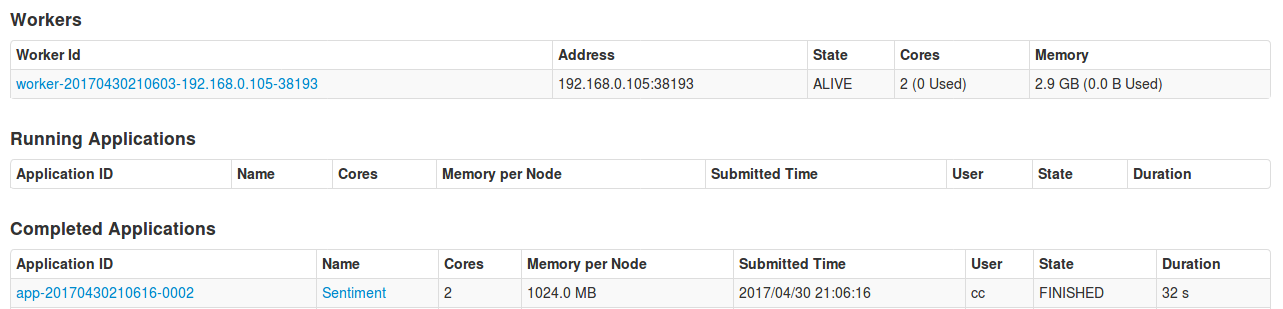
\includegraphics[width=\linewidth, height = 1.5     in]{images/bm2}}
\caption{Run time of Naive Bayes in 1-node cluster}
\label{fig:chamstat1}
\end{figure}
\begin{figure}[htbp]
\centering
\fbox{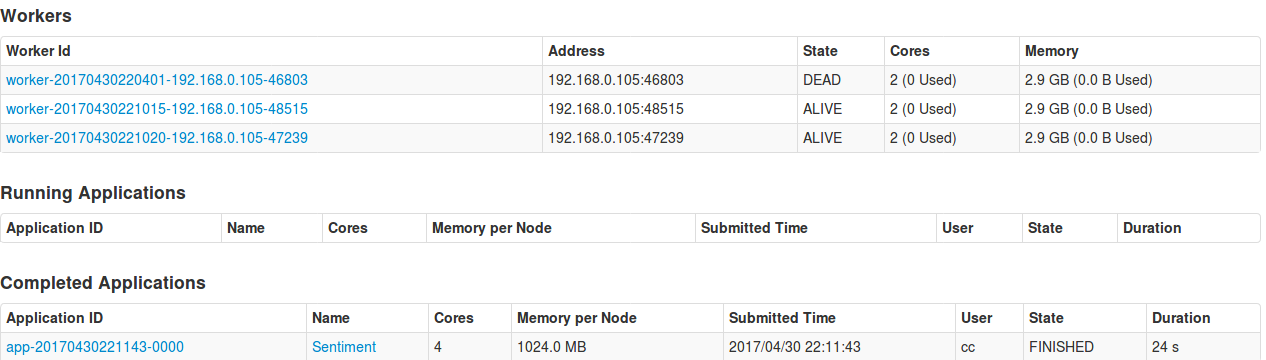
\includegraphics[width=\linewidth, height = 1.5     in]{images/bm1}}
\caption{Run time of Naive Bayes in 2-node cluster}
\label{fig:chamstat2}
\end{figure}
\begin{figure}[htbp]
\centering
\fbox{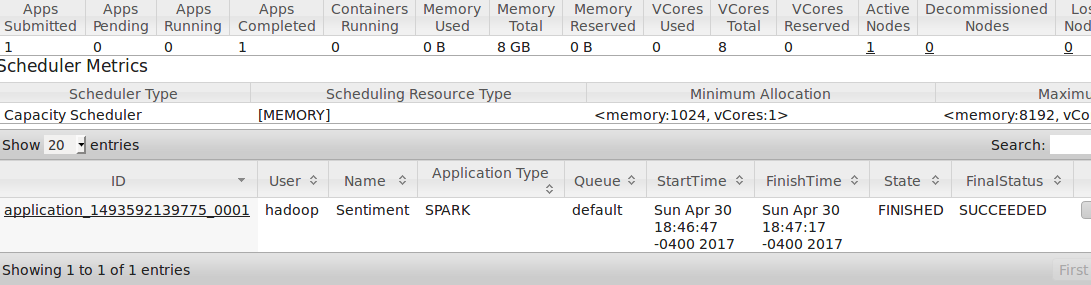
\includegraphics[width=\linewidth, height = 1.5     in]{images/bm3}}
\caption{Run time of Naive Bayes in 3-node cluster}
\label{fig:chamstat3}
\end{figure}
\subsubsection{Textbob}
\subsubsection{Naive Bayes}
\subsection{Jetstream}
\subsubsection{Textbob}
\subsubsection{Naive Bayes}
\subsection{Kilo}
\subsubsection{Textbob}
\subsubsection{Naive Bayes}
\section{Conclusion}
\paragraph{Acknowledgement}

Put in the information for this class and who may sponsor
you. Examples will be given later
\bibliography{references}
\end{document}
